This chapter will show the research that is undertaken before developing and designing the system. The main focus will be technical research as it will allowing me to find useful technologies that can be used to build the system. I will be analysing the existing system which will show what they are offering with their current system to their customers and also a public survey where it will show me if they are happy with the current system or what features they required in the new system. Through the use of an inventory check, this concept can provide an interactive solution for a local shop that cannot afford to pay higher fees.

\section{Existing Systems}
Before development, this is one of the most crucial steps that need to be taken in every project, therefore this will show us what is currently available in the market and what needs to be changed. To get the right aims and objective for the project, I have analysed a different system that is currently in the market. Most of the software has a similar feature with a decent User Interface(UI) rather than having an interactive UI where the user can feel more comfortable using the system. By analysing the current system will help me to find gaps in the design or functionality. Furthermore, all the feature they are available in the market are useful and I am making the same system with different design and service for local shopkeeper without monthly cost.\newline
\newline I have inspected various existing systems that are available in the market such as Dear Systems, Cin7, and Unleashed.

\subsection{Dear Systems}
Dear Systems is an inventory software that offers a point of sale(POS), Inventory management, financial management, and warehousing. The POS system that they offer is compatible with Android, PC, or Mac. Overall I like the system and services they offer but when you check out their monthly cost where they don't give this service to small business with 1 user. The cost for this system is \$199 per month and \$2189 per annual with 5 users.   

\subsection{Cin7}
Cin7 is one of the most popular management systems that are available in the market. It is fully integrated with point of sale (POS) and inventory management system where they have a real-time tracking system on inventory and sales. It is very difficult to tell the exact cost of the software as the company only gives the price by quote. The system comes with the manned tills where heir software is installed and connected with the inventory. The system also has reporting features where the user can check the inventory level, top-selling item, profit, losses, cost of goods, etc. Overall the color theme of the UI seems boring as the users only interact with the site when the application has good UI. It is hard to tell what will be the monthly cost but some websites claim it starts from £199 per month for basic users. If I were a shop keeper who owns a retail business then i would not afford to pay the cost.

\subsection{Unleashed}
Unleashed has to be one of the most visited software used by big businesses with the various warehouse. It allows the user to get access to real-time data on stocks, costs, and tracking information. Real-time tracking gives accurate information on the user screen where you look at the item. They offer three different plans such as Medium, Large and Large plus. All these plans have various monthly costs such as Medium cost £149, Large cost £299 and Large plus cost £519. All these costs are higher and cannot be afforded by local shop therefore I am making this inventory software to help them not to pay any fees.    

\section{Back-end Software}
It involves the choice of correct back-end software which enables me to store the data in a database using PHP and MySQL. This data will be retrieved and show the information right back into the user browser. I will be comparing two different software such as MongoDB and MySQL.

\subsection{MongoDB}
It is an open-source document-based database management program. It was used by many organisations such as Twitter, Sony, Zen desk, etc. It stores the data in JSON- like documents that can have varied structure. It does not use the usual rows and column format where we see in the relational database in MySQL. It does not require to declare the structure of documents to the system. 

\subsection{MySQL}
It is an open-source relational database management system(RDMS). It stores data in the form of rows of a table and uses the structured query language to access the data. It required me to define the tables and columns before I store any data and every row in the table needs to have the same columns. I was more familiar with MySQL language as I have used this language before in other projects therefore I will be using MySQL databases for my Inventory check system.

\section{Libraries}
I have evaluated two particular libraries before developing any software. jQuery developed by the jQuery Team and bootstrap 4 developed by Bootstrap Core Team for helping with front-end web development.

\newpage
\subsection{jQuery}
jQuery is a JavaScript library that allows users to add functionality to the website. It works in most of the web browsers that are available in the market. This will help to create my UI such as animating, event handling, etc. I have used this library to make a confirmation dialog box for the contact form. The following code is an example of a jquery library that I have used in the contact form:
\begin{figure}[h]
\centering
    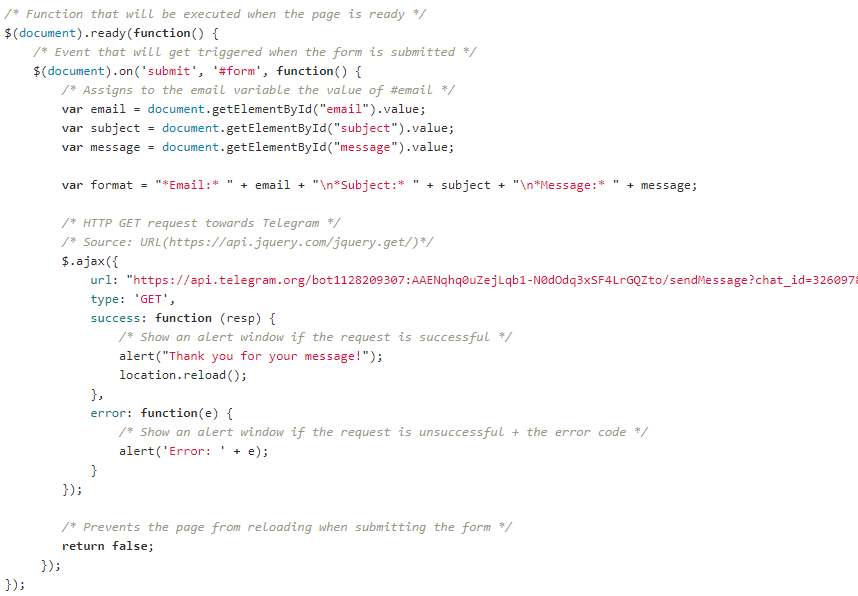
\includegraphics[scale=0.7]
    {images/contact.png}
    \caption{Contact form functionality using jQuery API }
    \label{fig: Contact form functionality using jQuery API}
\end{figure}

\newpage
\subsection{Bootstrap 4}
It is an open-source front-end development framework. It has many different interface components such as navigation, forms, model, Buttons, and more. It is one of the latest version with stable UI, I have used this framework to build a flexible, mobile-friendly, and responsive website. This framework does not have any issues to work in multiple browsers. It has saved me a lot of time and effort as it has predefined classes, tables, and other models. By saving time, I can give more time to other complicated work in other development work. I have learned this framework while I was working in college. The following code is one of the examples where I have used bootstrap:
\begin{figure}[h]
\centering
    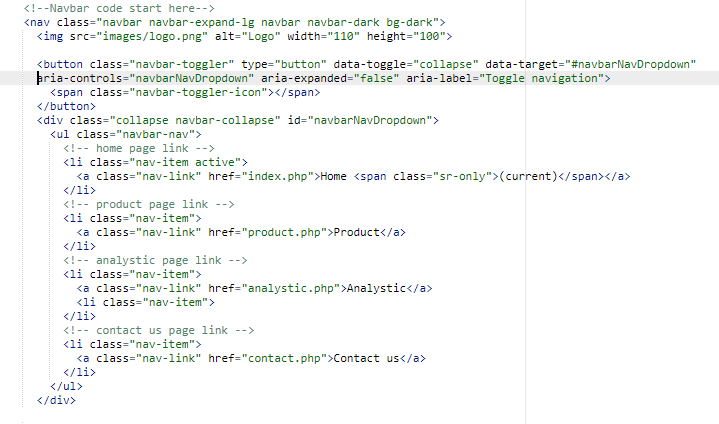
\includegraphics[scale=0.7]
    {images/navbar.png}
    \caption{Navbar using bootstrap framework}
    \label{fig: Navbar using bootstrap framework}
\end{figure}

\newpage
\section{Software Architecture}
To aid with selecting the best code editor, two editors were analysed such as brackets and sublime text to discover the hidden features.

\subsection{Brackets}
It is a source code editor that helps the developer to write the code and created by Adobe Systems. It is the useful editor as it shows live preview your code where you have written in HTML, CSS, and JavaScript. The main features it has is extracted which allows user to extract the information from fonts, colors straight from PSDs as clean CSS. I have chosen not to use brackets to write my code as it does not a feature for command line where I can manage my git repository and also run MySQL databases. 

\subsection{Sublime Text}
It is a source code editor that helps the developer to write the code in many different languages. It is one of my favorites text editor where I can use the command line to manage my git repository and also I can run my MySQL database directly from this editor. It is totally user friendly where you can modify multiple lines and look for specific code easily.

\section{Questionnaire/Survey Result}
Before developing an application, A survey was carried out to find out what they are looking for once the software has been developed. This survey was answered by my uncle and other local shopkeepers near my house. By making the questionnaire will help me to get a better understanding of the system they are using and how much do they pay. I have used the google form to create the questionnaire because, in the end, it will show me the result in the pie chart format. The full details of this survey can be found in the appendix A - Questionnaire/Survey Result.\newline
\newline Figure 2.3 clearly shows that 70\% of the people already using some kind of system that helps them to manage their inventory. This shows that shopkeepers love to use a management system.
\newpage
\begin{figure}[h]
\centering
    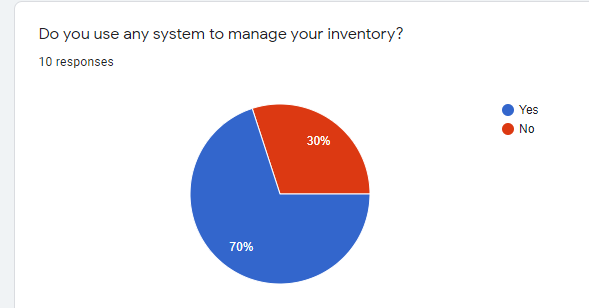
\includegraphics[scale=0.7]
    {images/SurveyQue1.png}
    \caption{Question 1: Use any system}
    \label{fig: Question 1: Use any system}
\end{figure}

Figure 2.4 shows that 50\% of the are using a spreadsheet to manage their inventory stocks and 37.5\% of people do not use any system instead they use paper to manage. This shows that they need a stable system that can manage their stocks online.
\begin{figure}[h]
\centering
    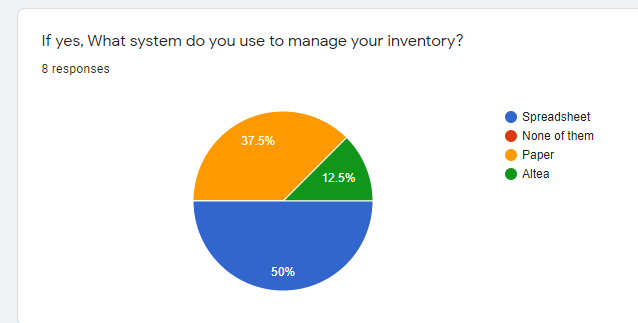
\includegraphics[scale=0.7]
    {images/SurveyQue2.png}
    \caption{Question 2: choose of system}
    \label{fig: Question 2: Use any system}
\end{figure}

\newpage 
Figure 2.5 shows that 70\% of the people do not pay any fees because they used a spreadsheet to manage their inventory and it does not cost anything. Whereas 30\% of the people pay between £51 - £100 Monthly and it was the cheapest cost that they found in the market. They were so happy when I told them that I am making a system to help them with no monthly cost.
\begin{figure}[h]
\centering
    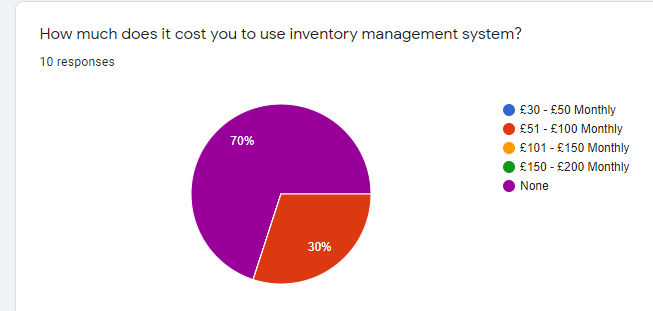
\includegraphics[scale=0.6]
    {images/SurveyQue3.png}
    \caption{Question 3: cost of current system}
    \label{fig: Question 3: cost of current system}
\end{figure}

Figure 2.6 shows that 50\% of the people use the spreadsheet daily and 50\% of people use weekly. This shows that they use the system to amend the stocks one a week or daily. Therefore my system will save their time and get the report on daily bases.
\begin{figure}[h]
\centering
    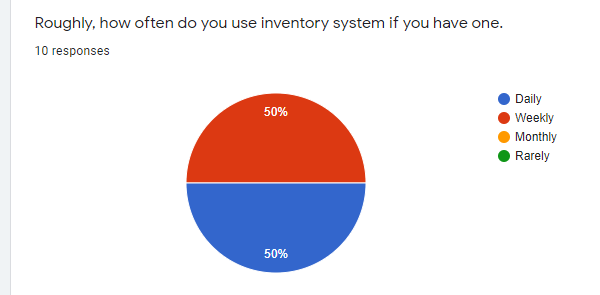
\includegraphics[scale=0.6]
    {images/SurveyQue4.png}
    \caption{Question 4: Usage of the system}
    \label{fig: Question 4: Usage of the system}
\end{figure}

\newpage
Figure 2.7 was asked to understand if the user will use the system for free and also if they like to use the system from anywhere in the world. It shows that out of 10 people, 90\% of them will use my system for free and 100\% of the people will use it from outside their shop or from a different country.
\begin{figure}[h]
\centering
    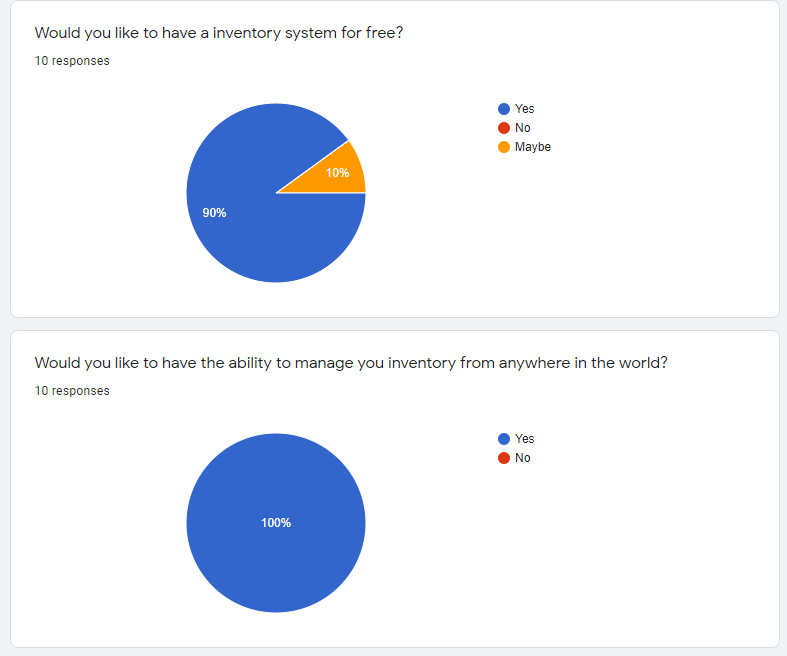
\includegraphics[scale=0.7]
    {images/SurveyQue5.png}
    \caption{Question 5 \& 6: Use the system for free and the ability to manage online}
    \label{fig: Question 5\& 6: Use the system for free and the ability to manage online}
\end{figure}

\newpage
Figure 2.8 shows that out of 10 people, 90\% of the people prefer to use my system to manage the inventory. This shows that I need to make a better and secure system. Therefore I need to give more time to my implementation.

\begin{figure}[h]
\centering
    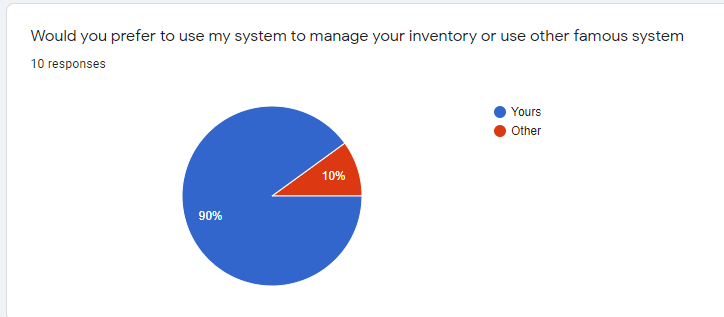
\includegraphics[scale=0.7]
    {images/SurveyQue7.png}
    \caption{Question 7: Prefer to use my system or other}
    \label{fig: Question 7: Prefer to use my system or other}
\end{figure}

\section{Project Aims}
This project aims for three main components which will help to build the system. The first layer in programming called the presentation layer which is responsible for delivery and formatting to the system. The second layer will act as a communication between the interface and the server. The final layer is a database that will store and retrieve the data to the user. I will be writing about three various layers such as front-end, Server-side(PHP), and Database server.

\subsection{Front-end}
\begin{enumerate}
    \item Easy to navigate throughout the website.
    \item Right choice of color to make the website interactive to the user.
    \item Able to show all the relevant data on the user screen.
    \item Show the product information when the user uses search functionality.
    \item Lock the important pages using the login and logout method.
    \item Ensure users can edit or delete the product.
\end{enumerate}

\subsection{Server-side (PHP)}
\begin{enumerate}
    \item Get the data from POST and GET method.
    \item Submit the MySQL query into the database when submitted by the user.
    \item Handle multiple request from the user.
\end{enumerate}

\subsection{Database server}
\begin{enumerate}
    \item Store and retrieve the data when required.
    \item Keep the table name up to date with the right key (Primary or Foreign Key).
    \item Able to submit the data when the user adds the product in the database.
\end{enumerate}